\begin{frame}{Secret Sharing $L_\infty$ ball}
    \begin{itemize}
        \item For center $(x_1, \ldots, x_d)$, we want to secret share this huge $L_\infty$ ball:
        \begin{equation*}
            [x_1 - \delta, x_1 + \delta] \times [x_2 - \delta, x_2 + \delta] \times \ldots \times [x_n - \delta, x_n + \delta]
        \end{equation*}

        \visible<2>{
        \item We can secret share each dimension separately, then AND the results.
        \begin{equation*}
            y_1 \ge x_1 - \delta \quad \wedge \quad y_1 \le x_1 + \delta \quad \wedge \quad \ldots \quad \wedge \quad y_d \ge x_d - \delta \quad \wedge \quad y_d \le x_d + \delta
        \end{equation*}
        }

    \end{itemize}

    \centering
    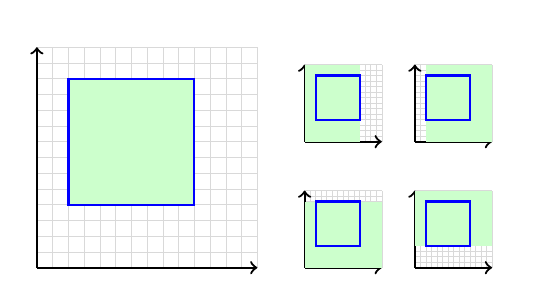
\begin{tikzpicture}[scale=0.4]
        % light grid
        \draw[step=0.5cm,gray!30,very thin] (0, 0) grid (7, 7);
    
        % axes
        \draw[->,thick] (0,0) -- (7,0) node[right] {};
        \draw[->,thick] (0,0) -- (0,7) node[above] {};
    
        % square with corners (1,2) and (5,6)
        \draw[thick,blue,fill=green!20] (1,2) rectangle (5,6);
    
        % optional: mark the corners
        % \filldraw[blue] (1,2) circle (2pt);
        % \filldraw[blue] (5,6) circle (2pt);
    
        % small planes on the right (2x2)
        \visible<2>{
        \begin{scope}[xshift=8.5cm,yshift=4cm,scale=0.35]
            \draw[step=0.5cm,gray!30,very thin] (0, 0) grid (7, 7);
            \draw[->,thick] (0,0) -- (7,0) node[right] {};
            \draw[->,thick] (0,0) -- (0,7) node[above] {};
            \fill[green!20] (0,0) rectangle (5,7);
            \draw[thick,blue] (1,2) rectangle (5,6);
        \end{scope}
        \begin{scope}[xshift=12cm,yshift=4cm,scale=0.35]
            \draw[step=0.5cm,gray!30,very thin] (0, 0) grid (7, 7);
            \draw[->,thick] (0,0) -- (7,0) node[right] {};
            \draw[->,thick] (0,0) -- (0,7) node[above] {};
            \fill[green!20] (1,0) rectangle (7,7);
            \draw[thick,blue] (1,2) rectangle (5,6);
        \end{scope}
        \begin{scope}[xshift=8.5cm,yshift=0cm,scale=0.35]
            \draw[step=0.5cm,gray!30,very thin] (0, 0) grid (7, 7);
            \draw[->,thick] (0,0) -- (7,0) node[right] {};
            \draw[->,thick] (0,0) -- (0,7) node[above] {};
            \fill[green!20] (0,0) rectangle (7,6);
            \draw[thick,blue] (1,2) rectangle (5,6);
        \end{scope}
        \begin{scope}[xshift=12cm,yshift=0cm,scale=0.35]
            \draw[step=0.5cm,gray!30,very thin] (0, 0) grid (7, 7);
            \draw[->,thick] (0,0) -- (7,0) node[right] {};
            \draw[->,thick] (0,0) -- (0,7) node[above] {};
            \fill[green!20] (0,2) rectangle (7,7);
            \draw[thick,blue] (1,2) rectangle (5,6);
        \end{scope}
        }
    \end{tikzpicture}

\end{frame}
% Note: In the script, state clearly that in this talk to keep things simple, we do not talk about overflow

\begin{frame}
    \frametitle{Primitive: Function Secret Sharing (FSS)}
    \begin{itemize}
        \item FSS was introduced in \cite{boyle2015function}, allowing to secret share a function $f$ between multiple parties.
        \item For domain bit length $u$, security parameter $\kappa$, payload bit length $v$, the key size is $O(u \cdot (\kappa + v))$ bits.
    \end{itemize}
    \begin{center}
    \begin{tikzpicture}[>=stealth,thick]
        \node[minimum width=1.5cm,minimum height=1.2cm,align=center] (interval) at (0,0) {$x \le a?$};
        \node (oracle) at (2,0) {\includegraphics[width=2.6cm]{images/crystal_ball_transparent.png}};
        \node (key1) at (8,1.4) {\includegraphics[width=1.8cm]{images/key_transparent.png}};
        \node (key0) at (8,-1.4) {\includegraphics[width=1.8cm]{images/key_transparent.png}};

        \draw[->] (interval.east) -- (oracle.west);
        \draw[->] (oracle.east) -- (key1.west);
        \draw[->] (oracle.east) -- (key0.west);

        \node at ([yshift=0pt]key1.north) {$k_1$};
        \node at ([yshift=0pt]key0.south) {$k_0$};
    \end{tikzpicture}
    \end{center}
\end{frame}

\begin{frame}
    \frametitle{Function Secret Sharing in \cite{garimella2024computation}}
    \begin{itemize}
        \item Alice prepares $O(\kappa)$ FSS keys pairs with \textit{binary output} (\textit{in} / \textit{out}?) for each inequality check.
        \item Alice and Bob runs 1-out-of-2 OTs, for Bob to learn either $k_0^i$ or $k_1^i$ for each inequality check.
        \item If the inequality check succeeds, for any of $\kappa$ key pairs, the evaluations would be equal.
    \end{itemize}
    \begin{center}
    \begin{tikzpicture}[>=stealth,thick,node distance=0.9cm and 1.4cm,xscale=0.95]
        \node[anchor=west] (alice) at (-1.2,2.6) {\includegraphics[height=1.6cm]{images/Alice_transparent.png}};
        \node (ineq) at (0,0) {$y_1 \ge x_1 - \delta\ ?$};

        % many key pairs for the single inequality check
        \foreach \i/\y in {1/2.0,2/0.8,3/-0.4,4/-1.6}{
            \node (k0\i) at (3,\y) {$k_0^{\i}$};
            \node (k1\i) at (4.8,\y) {$k_1^{\i}$};
            \draw[->] (ineq.east) -- (k0\i.west);
            \draw[->] (ineq.east) -- (k1\i.west);

            % Bob does 1-out-of-2 OT for each pair
            \node[draw,rounded corners,fill=gray!15,inner sep=4pt] (ot\i) at (7.2,\y) {OT pick 1};
            \draw[->] (k0\i.east) -- (ot\i.west);
            \draw[->] (k1\i.east) -- (ot\i.west);
        }

        \node[anchor=west] (bob) at (9.2,0) {\includegraphics[height=1.4cm]{images/Bob transparent.png}};
        \foreach \i/\y in {1/2.0,2/0.8,3/-0.4,4/-1.6}{
            \draw[->] (ot\i.east) -- (bob.west |- ot\i);
        }
    \end{tikzpicture}
    \end{center}
\end{frame}

\begin{frame}
    \frametitle{Can we use only one key pair?}
    \begin{itemize}
        \item Alice can prepare only one FSS key pair for each inequality check, with \textit{longer payload}.
        \item This will also avoid dictionary attack from Bob. 
        \item However, Alice can prepare malicious payload, which is undesirable.
        \item Nonetheless, the key size for one inequality check is improved:
    \end{itemize}
    \begin{center}
    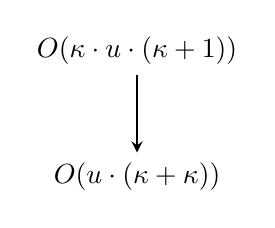
\begin{tikzpicture}[>=stealth,thick]
        \node (eqtop) at (0,0) {$O(\kappa \cdot u \cdot (\kappa + 1))$};
        \node (eqbottom) at (0,-1.6) {$O(u \cdot (\kappa + \kappa))$};
        \draw[->] (eqtop) -- (eqbottom);
    \end{tikzpicture}
    \end{center}
\end{frame}

\begin{frame}
    \frametitle{Distributed DCF}
\end{frame}